%\newcommand{\F}{\mathbb{F}}
%\newcommand{\G}{\mathbb{G}}
\newcommand{\Cdel}{\ensuremath{c_{del}}}
\newcommand{\Cins}{\ensuremath{c_{ins}}}
\newcommand{\Cupd}{\ensuremath{c_{upd}}}

\newcommand{\AfullDecomposition}{\ensuremath{\mathcal{A}}}
\newcommand{\FrelevantSubforests}{\ensuremath{\mathcal{F}}}
\newcommand{\pluseq}{\stackrel{+}{=}}
\newcommand{\AlgCase}{$\left\{\rule{0pt}{\baselineskip}\right.$\parbox{\textwidth}}

\newcommand{\rtedCostSum}[3]{\sum_{{#1}' \in #1 - \gamma^{#2}(#1)}cena({#1}', #3)}


%indentation in code:
\algdef{SE}[SUBALG]{Indent}{EndIndent}{}{\algorithmicend\ }
\algtext*{Indent}
\algtext*{EndIndent}


\chapter{Tree-edit-distance algoritmus}

Jadro aplikacie leží v použití tree-edit-distance (TED) algoritmu,
vďaka ktorému dostaneme mapovanie medzi 2 RNA stromami. Mapovanie nám ukáže
spoločné časti oboch RNA stromov. TED algoritmus je obdoba Levenstheinoveho
string-edit-distance algoritmu. Problém u reťazcov je špecialným prípadom
TED-u, kedy stromy zdegenerovali na cesty (spojový zoznam).

\section{Hlavná myšlienka TED-u}

Základ TED algoritmu je v rekurzivnom vzorci \ref{eq:ted} z \citet{DMRW} a \citet{RTED}. Vzdialenosť medzi
lesmi $F$ a $G$, $\delta(F, G)$ je definovana ako minimálny počet editačných operácií,
ktoré z F urobia G. Používame štandardne editačné operácie - delete, insert, update.

\begin{figure}[H]
\centering
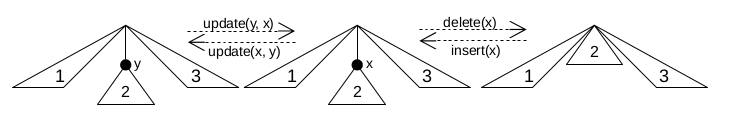
\includegraphics[width=140mm, height=30mm]{../img/TED_operations.png}
\caption{Ukazky TED operacii}
\label{obr:TED_operations}
\end{figure}

Delete, zmazanie vrcholu, znamená pripojiť k predkovi všetkých jeho potomkov so
zachovanim poradia medzi nimi. Insert, vložnie vrcholu, je opačná operácia k
delete, čo znamená, že vkladáme vrchol medzi rodiča a nejakých jeho, po sebe
nasledujúcich potomkov. Update iba zmeni hodnotu vo vrchole stromu.

\section{Značenie}

V tejto kapitole sa budeme riadiť značením \citet{RTED}. Teda, používame definiciu
stromu a lesa z \ref{def:strom}. Ak $F$ je les (strom), $N_F$ označuje množinu jeho vrcholov a $E_F$
množinu jeho hrán. Platí ďalej že $E_F \subseteq N_F \times N_F$. $\emptyset$ označuje
prázdny strom, resp. prázdny les. Podles lesa $F$ je graf $\tilde{F}$ s vrcholmi
$N_{\tilde{F}} \subseteq N_F$ a hranami $E_{\tilde{F}} \subseteq E_F \cap N_{\tilde{F}} \times N_{\tilde{F}}$.
Obdobne to platí aj pre podstrom stromu $T$.
$F_{v}$ označuje podstrom $F$ zakorenený vo $v$, t.j. v strome ostávajú iba potomkovia $v$.
$F - v$ budeme značiť les, ktorý dostaneme zmazaním vrcholu $v$ z $F$, spolu so všetkými hranami
zasahujúcimi do $v$. Podobne $F - F_{v}$ budeme značiť les, ktorý dostaneme zmazaním podstromu
$F_{v}$ z $F$.

\begin{definice}[Editačná vzdialenosť]
	Nech F a G sú dva lesy. Editačna vzdialenosť, tree-edit-distance - $\delta(F, G)$,
	medzi F a G je rovná minimálnej cene, za ktorú les F transformujeme na G.
\end{definice}

Vo vzorci \ref{eq:ted} počítame editačnú vzdialenosť $\delta(F, G)$,
\Cdel, \Cins a \Cupd sú ceny zmazania, vloženia a editácie vrcholu v strome
a $r_{F}$ a $r_{G}$ sú korene, buď obidva najpravejšie alebo najľavejšie (tzn. vyberieme
najpravejší/najľavejší strom lesa a jeho koreň).

\begin{figure}[H]
  \begin{subequations}
  \begin{align*}
    \begin{split}
    \delta(\emptyset, \emptyset) &=
      0
      \\
    \delta(F, \emptyset) &=
      \delta(F - r_{F}, \emptyset) + \Cdel(r_{F})
      \\
    \delta(\emptyset, G) &=
      \delta(\emptyset, G - r_{G}) + \Cins(r_{G})
    \end{split}
    \\[1ex]
    \delta(F, G) &=
      \begin{cases}
        \delta(F - r_{F}, G) + \Cdel(r_{F}) \\
        \delta(F, G - r_{G}) + \Cins(r_{G}) \\
        \delta(F - F_{r_{F}}, G - G_{r_{G}}) + \\
          \quad \delta(F_{r_{F}} - r_{F}, G_{r_{G}} - r_{G}) + \Cupd(r_{F}, r_{G})
      \end{cases}
  \end{align*}
  \end{subequations}
  \caption{Rekurzívny vzorec pre výpočet tree-edit-distance}
  \label{eq:ted}
\end{figure}


\section{Algoritmy dynamického programovania}

\citet{TAI} predstavil algoritmus s priestorovou a časovou zložitosťou \O{$m^3 \cdot n^3$},
\citet{ZHANGSHASHA} algoritmus následne vylepšili pozorovaním toho, že nepotrebujeme
vzdialenosti medzi všetkými pármi podlesov. Algoritmus mal časovú zložitosť \O{$m^2 \cdot n^2$}
a priestorovú \O{$m \cdot n$}. \citet{KLEIN} dosiahol časovú zložitosť \O{$m^2 \cdot n \cdot \log{n}$},
avšak jeho riešenie potrebovalo rovnako veľa pamäte.
\citet{DALUCQ} ukázali, že minimálny čas na beh algoritmu je \O{$m \cdot n \cdot \log{m} \cdot \log{n}$}.
\citet{DMRW} predviedli worst-case optimálny algoritmus pre tree-edit-distance.
Jeho časová a priestorová zložitosť je \O{$m^2 \cdot n \cdot (1 + \log{\frac{n}{m}})$} a
\O{$m \cdot n$}. \citet{RTED} ukázali spojitosť medzi efektivnosťou predchádzajúcich algoritmov
a tvarom stromov. Zovšeobecnili predchádzajúce prístupy a vytvorili algoritmus bežiaci
vo worst-case čase \O{$m^3$} a priestore \O{$m \cdot n$}. Ich algoritmus je teda efektívny pre všetky
tvary stromov a nikdy nespadne do worst-case, ak existuje lepší smer výpočtu. 



\subsection{RTED}

Ďalej sa v našej práci budeme venovať výhradne algoritmu RTED od tvorcov \citet{RTED}.
Ich algoritmus rozdelíme na 2 časti, rovnako pomenovaný RTED a GTED.

RTED (Robust Tree Edit Distance) algoritmus bude pre nás algoritmus na výpočet
optimálnej dekompozičnej stratégie (viz definicia \ref{def:strategy})
a GTED (General Tree Edit Distance) algoritmus samotný výpočet rekurzie \ref{eq:ted}
s aplikovaním danej stratégie.

\begin{definice}[Dekompozičná stratégia]\label{def:strategy}
	Nech $F$ a $G$ sú lesy. Dekompozičná stratégia v rekurzií \ref{eq:ted} priradí
  každej dvojici podstromov $F_{v}$ a $G_{w}$ lesov $F$ a $G$ jednu cestu $\gamma_{T}$
  z koreňa do listu, kde $T \in \{F, G\}$.
	LRH dekompozičná stratégia vyberá vždy najľavejší/najpravejší/najťažší
	(left/right/heavy) vrchol na ceste z koreňa do listu. Najťažší vrchol je taký,
	v ktorého podstrome je najviac vrcholov. 
\end{definice}

\subsubsection{GTED: General Tree Edit Distance algoritmu}

Začneme princípom fungovania GTED algoritmu. Detaily pre LRH stratégie sú
v \citet{ZHANGSHASHA} pre left/right a v \citet{DMRW} pre heavy stratégiu.

\begin{algorithm}
  \caption{General Tree Edit Distance for LRH strategies}
  \label{alg:gted}
  \begin{algorithmic}[1]
    \Procedure {gted}{$F, G, TreeDistance, S$}
      \State $\sigma \gets S[F, G]$
      \If {$\sigma \in \sigma^{*}(F)$}
        \ForAll {$F' \in F - \sigma$}
          \State $TreeDistance \gets TreeDistance \cup \Call{gted}{F', G, TreeDistance, S}$
        \EndFor
        \State $TreeDistance \gets TreeDistance \cup$
        \Indent
          \State $\Call{Compute Distance}{F, G, TreeDistance, \sigma}$
        \EndIndent
      \Else
        \State $TreeDistance \gets TreeDistance \cup (\Call{gted}{G, F, TreeDistance^{T}, S^{T}})^{T}$
      \EndIf
      \State \Return{$TreeDistance$}
    \EndProcedure
  \end{algorithmic}
\end{algorithm}

\begin{algorithm}
  \caption{Single path function}
  \label{alg:spf}
  \begin{algorithmic}[1]
    \Procedure {Compute Distance}{$F, G, TreeDistance, \sigma$}
      \If {$\sigma \in \sigma^{*}(F)$}
        \ForAll {$G' \in \Call{Relevant Subtrees}{G}$}
          \State $\Call{Single Path}{F, G', TreeDistance, \sigma}$
        \EndFor
      \Else
        \ForAll {$F' \in \Call{Relevant Subtrees}{F}$}
          \State $\Call{Single Path}{F, G, TreeDistance, \sigma}$
        \EndFor
      \EndIf
    \EndProcedure
    \\
    \Procedure {Single Path}{$F, G, TreeDistance, \sigma$}
      \State $ForestDistance \gets$ empty array $|F| + 1 \times |G| + 1$
      \State $ForestDistance[\emptyset][\emptyset] := 0$
      \For {$F'$ subforest in \Call{get ordered subforests}{$F, \sigma$}}
        \State $Last_{F} \gets$ last added node to $F'$
        \State $ForestDistance[F'][\emptyset] := ForestDistance[F' - Last_{F}][\emptyset] +$
        \Indent
          \State $C_{del}(Last_{F})$
        \EndIndent
      \EndFor
      \For {$G'$ subforest in \Call{get ordered subforests}{$G, \sigma$}}
        \State $Last_{G} \gets$ last added node to $G'$
        \State $ForestDistance[\emptyset][G'] := ForestDistance[\emptyset][G' - Last_{G}] +$
        \Indent
          \State $C_{ins}(Last_{G})$
        \EndIndent
      \EndFor
      \For {$F'$ subforest in \Call{get ordered subforests}{$F, \sigma$}}
        \For {$G'$ subforest in \Call{get ordered subforests}{$G, \sigma$}}
          \State $Last_{F} \gets$ last added node to $F'$
          \State $Last_{G} \gets$ last added node to $G'$
          \If {both $F'$ and $G'$ are trees}
          \label{alg:spf:iftrees}
            \State $C_{min} := min \{$
            \Indent
            \State $ForestDistance[F' - Last_{F}][G'] +$
              \Indent
                \State $C_{del}(Last_{F})$,
              \EndIndent
              \State $ForestDistance[F'][G' - Last_{G}] +$
              \Indent
                \State $C_{ins}(Last_{G})$,
              \EndIndent
              \State $ForestDistance[F' - Last_{F}][G' - Last_{G}] +$
              \Indent
                \State $C_{upd}(Last_{F}, Last_{G})$
              \EndIndent
            \EndIndent
            \State $ForestDistance[F', G'] := C_{min}$
            \State $TreeDistance[Last_{F}][Last_{G}] := C_{min}$
          \Else
          \label{alg:spf:ifforests}
            \State $C_{min} := min \{$
            \Indent
              \State $ForestDistance[F' - Last_{F})][G'] +$
              \Indent
                \State $C_{del}(Last_{F})$,
              \EndIndent
              \State $ForestDistance[F'][G' - Last_{G}] +$
              \Indent
                \State $C_{ins}(Last_{G})$,
              \EndIndent
              \State $ForestDistance[F' - F_{Last_{F}}][G' - G_{Last_{G}}] +$
              \Indent
                \State $TreeDistance[F_{Last_{F}}][G_{Last_{G}}]\}$
              \EndIndent
            \EndIndent
            \State $ForestDistance[F'][G'] := C_{min}$
          \EndIf
        \EndFor
      \EndFor
    \EndProcedure
  \end{algorithmic}
\end{algorithm}


\begin{pozn}
  Funkcia $Get Ordered Subforests()$ v algoritme \ref{alg:spf} vracia lesy zoradené
  v opačnom poradí, ako ich pridávame v definícii \ref{def:relevant_subforests}.
\end{pozn}

Algoritmus \ref{alg:gted} funguje v troch krokoch.

Najprv podľa stratégie dekomponuje jeden zo stromov podľa cesty $\gamma$,
bez ujmy na obecnosti, nech je to $F$ a rekurzívne spočíta editačnú vzdialenosť
medzi všetkými podstromami, ktoré susedia s dekompozicnou cestou a stromom $G$.

Následne pre všetky relevant-subtrees (viz definice \ref{def:relevant_subforests})
podstromy $G'$ stromu $G$ vyráta vzdialenosti medzi $F_{v}$ a $G'$ pomocou single-path funkcie.
Tá dopočíta vzdialenosti medzi vrcholmi $v \in \gamma_{F}$ a stromami $G'$.

\begin{definice}
  \label{def:relevant_subforests}
	Relevant subtrees stromu $F$ pre root-leaf cestu $\gamma$ sú definované ako $F - \gamma$.
	Relevant subforests stromu $F$ pre nejakú root-leaf cestu $\gamma$ sú definované rekurzívne ako
	\begin{align*}
    \mathcal{F}(\emptyset, \gamma) &= \emptyset
		\\
		\mathcal{F}(F, \gamma) &= \{F\} \cup
		\begin{cases}
      \mathcal{F}(F - r_{R}(F), \gamma), \quad{} &\text{ak $r_{L}(F) \in \gamma$}
			\\
      \mathcal{F}(F - r_{L}(F), \gamma), &\text{v ostatných pripadoch}
		\end{cases}
	\end{align*}
\end{definice}

\begin{lemma}
  Ak compute-distance funkcia dopočíta editačnú vzdialenosť medzi vrcholmi na ceste $\gamma$
  a všetkými podstromami druhého stromu, potom GTED vráti maticu vzdialenosti
  medzi všetkými dvojicami podstromov $F_{v}$ a $G_{w}$, pre $v \in F; w \in G$.
\end{lemma}

\begin{dukaz}
  Nech $\gamma \in F$. Po vyrátani editačnej vzdialenosti medzi stromami
  $F - \gamma$ a $G$ nám stačí dopočítať už len vrcholy na ceste,
  teda vzdialenosti medzi stromami $F_{v}$ a $G$ pre $v \in \gamma_{F}$.
\end{dukaz}

Vďaka doslednému usporiadaniu lesov si v každom kroku pripravíme potrebne
data pre ďalší krok algoritmu \ref{alg:spf}.

Najprv si ešte ale vysvetlíme hodnoty používané v algoritme \ref{alg:spf} v podmienkách
na riadkoch \ref{alg:spf:iftrees} a \ref{alg:spf:ifforests}. Prvé dva sú v oboch rovnaké.
Počítame hodnotu zmazania vrcholu z $F$, resp. vloženia vrcholu do $F$.

Tretia hodnota sa líši podľa toho, či sú lesy zároveň aj stromami. Ak sú, tak na danom mieste
je cena namapovania podstromov $F_{v} - v$ na $F_{w} - w$ a updatu vrcholu $v$ na $w$.
Inac, ked aspon jeden z lesov nieje stromom, tak cenu medzi $F_{Last_{F}}$ a $G_{Last_{G}}$
mame vyrátanú z predchádzajúcich krokoch, alebo z inej vetvy rekurzie.

Potom nastavíme hodnotu vzdialenosti medzi lesmi na minimum a v prípade že sú to obidva stromy,
tak nastavíme aj ich vzdialenosť.

Najprv ešte ukážeme, že SPF používa vždy inicializované hodnoty a každú hodnotu nastavuje práve raz.

\begin{pozn}
  Nikdy nepoužívam 2x rovnakú cestu $\gamma$ v strome. To vyplýva z toho, že po dekompozícií
  stromu podľa $\gamma$, cesta v ostatných stromoch neexistuje.
1\end{pozn}

\begin{pozn}
  Single-path funkcia každú hodnotu $ForestDistance$, rovnako ako $TreeDistance$ nastavuje
  práve raz.
\end{pozn}

\begin{dukaz}
  Žiadnu cestu nepoužívam opakovane. Hodnotu v $TreeDistance$ nastavujem iba v momente,
  keď sú obidva lesy stromami (teda ich korene ležia na cestách $\gamma_{F}$ a $\gamma_{G}$)
  a to sa udeje práve raz.
  Lesy vždy iba zväčšujem, takze nikdy sa nedostanem do menšieho aby som mohol mu znovu nastaviť
  hodnotu. To iste plati aj pre $ForestDistance$.
\end{dukaz}

\begin{lemma}
  Nikdy nepoužívame neinicializované hodnoty $TreeDistance$ a $ForestDistance$.
\end{lemma}

\begin{dukaz}
  Hodnota $ForestDistance$ pre použitie s prázdnym lesom je inicializovaná, a pri každej iteracií
  algoritmu čítam iba z hodnôt z predchadzajúcich iteracií, napr.
  $ForestDistance[F - Last_{F}][G - Last_{G}]$, alebo $ForestDistance[F - F_{Last_{F}}][G - G_{Last_{G}}]$.
  V prvom prípade mažem iba jeden vrchol, v druhom celý jeho podstrom.

  Hodnoty $TreeDistance$ používame iba v prípade, že aspoň jeden z lesov $F'$ alebo $G'$ nieje stromom.
  To znamená, že ak posledne pridaný vrchol $Last_{F}$ je mimo cesty $\gamma_{F}$, tak sme vzdialenosť
  od $Last_{G}$ vyrátali rekurzívne po dekompozicií $F$ už skôr.
  Naopak ak $Last_{F}$ leži na ceste, potom $Last_{G}$ je mimo cesty, a editačnú vzdialenosť
  sme vyrátali pri počítani relevant-subtrees.
\end{dukaz}

\begin{dusl}
  Algoritmus funguje.
\end{dusl}

\begin{dukaz}
  V predchádzajúcich častiach sme dokázali, že v každom kroku používame iba korektné hodnoty a
  všetky časti algoritmu počítajú správne, takže algoritmus GTED je v poriadku.
\end{dukaz}

%TODO priklad

\subsubsection{RTED: Robust Tree Edit Distance algoritmus}

RTED budeme vnímať ako algoritmus na výpočítanie optimálnej stratégie - teda algoritmus,
ktorý nám poradí ako najlepšie dekomponovať obidva stromy.

Funguje tak, že si predpočíta koľko podproblémov budeme musieť vyriešiť, ak použijeme stratégiu
$left$, $right$, alebo $heavy$.

\begin{definice}
	Celková dekompozícia lesa (full decomposition) $F$, $\mathcal{A}(F)$ je množina
	všetkych podlesov F, ktoré dostaneme rekurzívnym odstranením najľavejšieho
	alebo najpravejšieho koreňového vrcholu - $r_{R}(F)$ a $r_{L}(F)$ - z $F$
	a následne aj všetkých jeho podlesov.
	\begin{align*}
		\mathcal{A}(\emptyset) &= \emptyset
		\\
		\mathcal{A}(F) &= {F} \cup \mathcal{A}(F - r_{L}(F)) \cup \mathcal{A}(F - r_{R}(F))
	\end{align*}
\end{definice}

\begin{figure}[H]
\centering
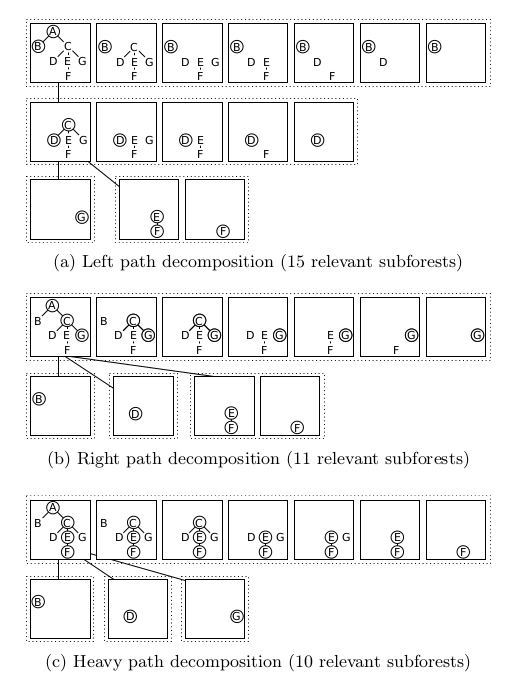
\includegraphics[width=85mm, height=100mm]{../img/LRH_decomposition.png}
%TODO vlastné obrázky
\caption{Celková dekompozícia pomocou LRH strategii}
\label{obr:LRH_decomposition}
\end{figure}

\begin{lemma}
  Počet podproblémov (relevant-subproblems) počítaných single-path funkciou pre dvojicu
  stromov $F$ a $G$ je rovná
  \begin{align*}
    \# = 
    \begin{cases}
      \abs{F} \times \abs{\FrelevantSubforests(G, \Gamma^{L}(G))} & \text{pre left-paths}
      \\
      \abs{F} \times \abs{\FrelevantSubforests(G, \Gamma^{R}(G))} & \text{pre right-paths}
      \\
      \abs{F} \times \abs{\AfullDecomposition(G)} & \text{pre heavy-paths}
    \end{cases}
  \end{align*}
\end{lemma}

\begin{dukaz}
  \citet{DMRW} dokázali, že vzorec pre ťažké cesty je v poriadku. Rovnako tak,
  \citet{ZHANGSHASHA} to dokázali pre ľavé cesty. Jednoduchou úpravou vieme upraviť
  ich vzorec na použitie pravých ciest.
\end{dukaz}

\begin{definice}
  Minimálny počet podproblémov, ktoré potrebujeme vyrátať pri použití GTEDu je
  \begin{align*}
    cena(F, G) =
    \begin{cases}
      \abs{F} \times \abs{\AfullDecomposition(G)} &+ \rtedCostSum{F}{H}{G}
      \\
      \abs{G} \times \abs{\AfullDecomposition(F)} &+ \rtedCostSum{G}{H}{F}
      \\
      \abs{F} \times \abs{\FrelevantSubforests(G, \Gamma^{L}(G))} &+ \rtedCostSum{F}{L}{G}
      \\
      \abs{G} \times \abs{\FrelevantSubforests(F, \Gamma^{L}(F))} &+ \rtedCostSum{G}{L}{F}
      \\
      \abs{F} \times \abs{\FrelevantSubforests(G, \Gamma^{R}(G))} &+ \rtedCostSum{F}{R}{G}
      \\
      \abs{G} \times \abs{\FrelevantSubforests(F, \Gamma^{R}(F))} &+ \rtedCostSum{G}{R}{F}
    \end{cases}
  \end{align*}
\end{definice}

\begin{dukaz}
  je uvedený v \citet{RTED}
\end{dukaz}

Namiesto \O{$n^3$} rekurzie potrebujeme algoritmus, ktorý optimálnu stratégiu vyráta
s nižšími časovými nárokmi ako potrebuje optimálny beh $GTED$u.

Popiseme teda algoritmus \ref{alg:rted} - RTED, od tvorcov \citet{RTED}.
Bežiaci v čase \O{$n^2$}.

\begin{algorithm}
  \caption{Optimálna stratégia}
  \label{alg:rted}
  \begin{algorithmic}[1]
    \Procedure {rted}{$F, G$}
      \State $L_{v}, R_{v}, H_{v} \gets$ polia velkosti $\abs{F} \times \abs{G}$
      \State $L_{w}, R_{w}, H_{w} \gets$ polia velkosti $\abs{G}$
      \ForAll {$v$ postorder v $F$}
        \ForAll {$w$ postorder v $G$}
          \If {$v$ je list}
            \State $L_{v}[v, w] \gets R_{v}[v, w] \gets H_{v}[v, w] \gets 0$
          \EndIf
          \If {$w$ je list}
            \State $L_{w}[w] \gets R_{w}[w] \gets  H_{w}[w] \gets 0$
          \EndIf

          \State $C := \{$
            \Indent
              \State $(\abs{F_{v}} \times \AfullDecomposition(G_{w}) +
                H_{v}[v, w], \gamma^{H}(F)),$
              \State $(\abs{G_{w}} \times \AfullDecomposition(F_{v}) +
                H_{w}[w], \gamma^{H}(G)),$
              \State $(\abs{F_{v}} \times
                \abs{\FrelevantSubforests(G_{w}, \Gamma^{L}(G))} +
                L_{v}[v, w], \gamma^{L}(F)),$
              \State $(\abs{G_{w}} \times
                \abs{\FrelevantSubforests(F_{v}, \Gamma^{L}(F)}) +
                L_{w}[w], \gamma^{L}(G)),$
              \State $(\abs{F_{v}} \times
                \abs{\FrelevantSubforests(G_{w}, \Gamma^{R}(G))} +
                R_{v}[v, w], \gamma^{R}(F)),$
              \State $(\abs{G_{w}} \times
                \abs{\FrelevantSubforests(F_{v}, \Gamma^{R}(F))} +
                R_{w}[w], \gamma^{R}(G))$
              \State $\}$
            \EndIndent

            \State $(c_{min}, \gamma_{min}) \gets (c, \gamma)$ take, ze
              $(c, \gamma) \in C \wedge c = min\{c' | (c', \gamma) \in C\}$
            \State $Strategies[v, w] := \gamma_{min}$

            \If {$v$ nieje koren}
            \State \Call{update}{$L_{v}$, v, w, $c_{min}$, $\gamma^{L}(parent(v)$}
              \State \Call{update}{$R_{v}$, v, w, $c_{min}$, $\gamma^{R}(parent(v)$}
              \State \Call{update}{$H_{v}$, v, w, $c_{min}$, $\gamma^{H}(parent(v)$}
            \EndIf
            \If {$w$ nieje koren}
              \State \Call{update}{$L_{w}$, w, $c_{min}$, $\gamma^{L}(parent(w)$}
              \State \Call{update}{$R_{w}$, w, $c_{min}$, $\gamma^{R}(parent(w)$}
              \State \Call{update}{$H_{w}$, w, $c_{min}$, $\gamma^{H}(parent(w)$}
            \EndIf
        \EndFor
      \EndFor
      \State \Return {$Strategies$}
    \EndProcedure

  \item[]

    \Procedure {update}{$Table, v, w, c_{min}, \gamma$}
      \State $Table[parent(v), w] \pluseq
        \begin{cases}
          Table[v, w] & \text{ak $v \in \gamma$}
          \\
          c_{min} & \text{v opacnom pripade}
        \end{cases}$
    \EndProcedure

    \Procedure {update}{$Table, w, c_{min}, \gamma$}
      \State $Table[parent(w)] \pluseq
        \begin{cases}
          Table[w] & \text{ak $v \in \gamma$}
          \\
          c_{min} & \text{v opacnom pripade}
        \end{cases}$
    \EndProcedure
  \end{algorithmic}
\end{algorithm}

Prechádza vrcholmi v postorder, aby sa znížila pamäťová náročnosť algoritmu a nemuseli ukladať hodnoty
medzi dvojicami relevant-subforest. Namiesto toho inkrementujeme hodnotu v rodičovskom vrchole pri
každej návšteve jeho potomka.

\begin{lemma}
  Algoritmus \ref{alg:rted} vyráta optimalnú LRH stratégiu pre dvojicu podstromov $F$ a $G$ a
  časová náročnosť algoritmu je \O{$n^2$}.
\end{lemma}

\begin{dukaz}
  Toto tvrdenie dokázali \citet{RTED}.
\end{dukaz}


\section{Mapovanie medzi stromami}

Tabuľka vzdialenosti z $GTED$u medzi stromami $F$ a $G$ nám nebude stačiť.
Potrebujeme vedieť ako strom $F$ namapovať na $G$.

\begin{algorithm}
  \caption{Počitanie mapovania}
  \label{alg:ted:mapping}
  \begin{algorithmic}[1]
    \Procedure {Mapping}{$F, G, TreeDistance$}
      \State $\sigma \gets$ lubovolna LRH strategia
      \State $ForestDistance \gets \Call{Single Path}{F, G, TreeDistance, \sigma}$
      \While {$F \neq \emptyset \wedge G \neq \emptyset$}
        \State $v \gets \Call{Update}{F, \sigma}$
        \State $w \gets \Call{Update}{G, \sigma}$
        \If {$ForestDistance[F, G] = ForestDistance[F - v, G] + C_{del}$}
          \State $Mapping \gets Mapping \cup (v \rightarrow 0)$
          \State $F \gets F - v$
        \ElsIf {$ForestDistance[F, G] = ForestDistance[F, G - w] + C_{ins}$}
          \State $Mapping \gets Mapping \cup (0 \rightarrow w)$
          \State $G \gets G - w$
        \Else
          \If {$F$ a $G$ su stromy}
            \State $Mapping \gets Mapping \cup (v \rightarrow w)$
            \State $F \gets F - v$
            \State $G \gets G - w$
          \Else
            \State $Mapping \gets Mapping \cup$
            \Indent
              \State $\Call{Mapping}{F - F_{v}, G - G_{w}, TreeDistance}$
            \EndIndent
            \State $F \gets F - F_{v}$
            \State $G \gets G - G_{w}$
          \EndIf
        \EndIf
      \EndWhile
    \EndProcedure
  \item[]
    \Procedure {Update}{$Forest, \sigma$}
      \State $\gamma \gets$ cesta v lese $Forest$ podla strategie $\sigma$
      \State \Return vrchol $r_{L}(Forest)$ alebo $r_{R}(Forest)$ alebo
        $\emptyset$ z $Forest$
        \Indent
          \State rovnako ako v definícií \ref{def:relevant_subforests}
        \EndIndent
      \label{alg:ted:mapping:update}
    \EndProcedure
  \end{algorithmic}
\end{algorithm}

Princíp je v backtrackovani matice $ForestDistance$, teda zisťujeme, akú operáciu, sme v ktorom
bode použili, podobne ako v zisťovaní operácií pri editačnej vzdialenosti reťazcov.
Musíme ale používať $ForestDistance$ maticu, nie $TreeDistance$, keďže v nej
sa odzrkadluje detailnejšia štruktúra stromov. Maticu $TreeDistance$ používame iba na
počítanie single-path funkcie.



